\documentclass[aps,prd,reprint,nofootinbib, superscriptaddress]{revtex4-1}
\usepackage{amsmath,amssymb, amsthm,amstext}
\usepackage{natbib}
\usepackage{graphicx}
\usepackage{color}
\usepackage{array, enumerate}
\usepackage{bm}
\usepackage{multirow}
\usepackage[breaklinks,colorlinks,citecolor=blue]{hyperref}


% Shorts
\def\nn{\nonumber}
\def\st{\sin\theta}
\def\ct{\cos\theta}
\def\sst{\sin^2\theta}
\def\cct{\cos^2\theta}
\def\Ap{A_\phi}
\def\Ar{A_{\phi,r}}
\def\Arr{A_{\phi,rr}}
\def\Am{A_{\phi,\mu}}
\def\Amm{A_{\phi,\mu\mu}}
\def\Ah{A_{\phi,\theta}}
\def\be{\begin{equation}}
\def\ee{\end{equation}}
\def\ben{\begin{eqnarray}}
\def\een{\end{eqnarray}}
\def\WH{\Omega_{\rm H}}
\def\e{{\bf e}}
\def\AHE{A_\phi^{\rm HE}}
\def\AEE{A_\phi^{\rm EE}}


\def\Alfven{Alfv\`en}


\begin{document}
\title{The force-free magnetosphere of a Kerr black hole: the role of boundary conditions}
\author{Zhen Pan}
\email{zhpan@ucdavis.edu}
\affiliation{Perimeter Institute for Theoretical Physics, Waterloo, Ontario N2L 2Y5, Canada}

\date{\today}

\begin{abstract}
    The role of boundary conditions in the structure of
    a force-free black hole magnetosphere was rarely discussed, since previous studies have been focused on the
    the field lines entering the horizon which is causally disconnected and on which the boundary
    condition imposed usually makes no difference to the magnetosphere structure. However,
    recent high-resolution general relativistic (GR) force-free simulation shows that there are both
    field lines entering the horizon and field lines ending up on the equatorial current sheet
    within the ergosphere for asymptotic uniform field. For the latter, the equatorial boundary
    condition is well approximated being marginally force-free, i.e., $B^2-E^2=0$, where $B$ and
    $E$ are the magnetic and electric field strength, respectively. In this paper, we revisit this
    problem by solving the GR Grad-Shafranov equation which governs the structure of
    the force-free magnetosphere in steady state and self-consistently imposing the marginally force-free equatorial
    condition. We also discuss the applicability of this boundary condition and the numerical algorithm proposed
    in this paper for general magnetic field configurations.
\end{abstract}


\maketitle

\section{Introduction}

\section{basic equations}
\label{sec:basic}
In this paper, we adopt the Kerr-Schild
coordinate with the line element
\[
\begin{aligned}
ds^2 =
&-\left( 1-\frac{2r}{\Sigma} \right)dt^2 + \left( \frac{4
r}{\Sigma} \right) dr dt + \left(1+\frac{2r}{\Sigma} \right) dr^2 \\
&+ \Sigma d\theta^2 - \frac{4 a r \sin^2\theta}{\Sigma} d\phi dt
- 2 a \left(1+\frac{2r}{\Sigma}\right) \sin^2\theta d\phi dr     \\
& + \frac{\beta}{\Sigma} \sst d\phi^2
\end{aligned}
\]
where $\Sigma = r^2 + a^2 \mu^2$, $\Delta = r^2 -2r + a^2$,
$\beta = \Delta\Sigma + 2r(r^2 + a^2)$, and $a$ is the dimensionless BH spin.
In the force-free approximation, electromagnetic energy greatly exceeds that of matter.
Consequently, the force-free magnetospheres is governed by energy
conservation equation of electromagnetic field, or
conventionally called as the GS equation.
In the Kerr spacetime,
the axisymmetric and steady GS equation can be written in a compact form \cite{Pan2017}
\ben
\label{eq:GSg}
&&\phantom{+}
 \left[\Arr + \frac{\sst}{\Delta}\Amm \right]  \mathcal K(r,\theta; \Omega )\nn \\
&&
+\left[\Ar \partial_r^\Omega  +  \frac{\sst}{\Delta}\Am \partial_\mu^\Omega\right] \mathcal K(r,\theta; \Omega ) \nn \\
&&
+ \frac{1}{2}\left[\Ar^2 + \frac{\sst}{\Delta}\Am^2\right]  \Omega' \partial_\Omega \mathcal K(r,\theta; \Omega )\nn \\
&&
- \frac{\Sigma}{\Delta}II' = 0 \ ,
\een
with $\mathcal K(r,\theta; \Omega )= \left[\frac{\beta}{\Sigma}\Omega^2 \sst
-\frac{4ra}{\Sigma}\Omega \sst
-\left(1-\frac{2r}{\Sigma}\right)\right]$ being the LS function,
$\mu\equiv\ct$,  and  the primes designate  derivatives with respect to $A_\phi$.
$\partial_i^\Omega (i=r, \mu)$  denotes the partial derivative
with respect to coordinate $i$ with $\Omega$ fixed, and $\partial_\Omega$ is the derivative with
respect to $\Omega$.

\section{Uniform field solution}

\subsection{Boundary conditions}

The boundary conditions on the polar axis, on the horizon and at infinity are natural.

\begin{subequations}
\begin{align}
    A_\phi(\mu = 1) &= 0,  \label{eq:bc1}\\
    \Am(\mu = 0, r > 2) &= 0, \label{eq:bc2}\\
    B^2-E^2 (\mu = 0, r_+ \leq r \leq 2) &=0.\label{eq:bc3}
\end{align}
\end{subequations}
where $r_+$ is the radius of the event horizon.

In our computation, we use following numerical prescription
\be
\label{eq:nbc}
\int_{A_\phi^{\rm HE}}^{A_\phi^{\rm EE}} \frac{B^2-E^2}{B^2+E^2} dA_\phi \Big/ \left(A_\phi^{\rm EE}- A_\phi^{\rm HE}\right)  < 10^{-3}.
\ee
as a proxy of the marginally force-free equatorial boundary condition (\ref{eq:bc3}),
where ``HE" and ``EE" are short for Horizon-Equator and Ergosphere-Equator, respectively.
Specifically,
\be
\begin{aligned}
B^2-E^2 &= \frac{1}{\Sigma \sst} \left[ -\mathcal{K} \left(\Ar^2 +\frac{\sst}{\Delta}\Am^2 \right)+\frac{\Sigma}{\Delta}I^2\right]\\
B^2+E^2 &= \frac{1}{\Sigma \sst} \left[ \left(\mathcal{K}+\frac{\Delta\Sigma}{\beta} \right) \left(\Ar^2 +\frac{\sst}{\Delta}\Am^2 \right)+\frac{\Sigma}{\Delta}I^2\right]\\
\end{aligned}
\ee
where $B^2+E^2$ is the energy density measured by the zero-angular-momentum-observers.

\subsection{Numerical method}
We aim to find a pair of $\Omega(A_\phi)$ and $I(A_\phi)$ satisfying the radiation condition
\be I = 2\Omega A_\phi, \label{eq:rad}\ee
enabling field lines smoothly crossing the LS,
and suitable normal derivative $\Am(\mu =0, r_+\leq r \leq 2)$ on the equator
guaranteeing the boundary condition (\ref{eq:bc3}).

In our computation, we define a new radial coordinate $R=r/(1+r)$, confine our
computation domain $R\times \mu$ in the region $[R(r_+), 1]\times [0,1]$,
and implement a uniform $512\times 64$ grid. The detailed algorithm is listed as follows.

1. We choose an initial guess for the field configuration, $\Omega(\Ap)$, $I(\Ap)$
and equator boundary condition as follows
\begin{subequations}
\begin{align}
    \Ap &= r^2 \sst,  \label{eq:gss1} \\
    \Omega & = 0.5\WH\left(1-\Ap/\AHE\right),  \label{eq:gss2}\\
    I & = \WH \Ap\left(1-\Ap/\AHE\right) , \\
    \Am(\mu =0, r_+\leq r \leq 2) & = - (r/r_+)^3, \label{eq:gss3}
\end{align}
\end{subequations}
where $\WH = a/2r_+$ is the BH angular velocity.

2. We evolve the GS equation (\ref{eq:GSg}) and adjust $II'(\Ap)$ enabling smooth field lines across the LS
\cite[see e.g.][for details]{Contopoulos2013, Nathanail2014, Pan2016a, Mahlmann2018}.

3. Usually the current $I$ found in Step 2 neither satisfies the radiation condition (\ref{eq:rad})
nor guarantees the boundary condition (\ref{eq:bc3}). We find it is possible to adjust
$\Am(\mu = 0, r_+ \leq r\leq 2)$ as follows
\be
 A_{\phi,\mu}|_{\rm new}  = A_{\phi,\mu}|_{\rm old} + \zeta_1\times[2\Omega\Ap(2\Omega\Ap)' -II'],
\ee
enabling the radiation condition (\ref{eq:rad}) for
$A_\phi\in [A_\phi^{\rm HE}, A_\phi^{\rm EE}]$, where $\zeta_1$ is an
empirical step size.

4. The remaining task is to adjust  $\Omega(0< \Ap < \AHE)$ enabling  the radiation condition (\ref{eq:rad})
 for $A_\phi \in (0, A_\phi^{\rm HE})$ and  to adjust $\Omega(\AHE \leq \Ap \leq \AEE)$
 enabling the boundary condition (\ref{eq:bc3}) for $\Ap \in [\AHE, \AEE]$.
 The first part is straightforward, i.e.,
 \be
\Omega_{\rm new} = \frac{I}{2\Ap}\Bigg|_{0 < \Ap < \AHE},
 \ee
 and the second part can be realized by
 \be
\Omega_{\rm new}  = \Omega_{\rm old} - \zeta_2\times\frac{\Delta (B^2-E^2)}{2\Ap}\Bigg|_{\mu=0, r_+\leq r \leq 2},
 \ee
 where $\zeta_2$ is again an empirical step size, and we have multiplied factor $\Delta$
 in the correction term to avoid numerical difficulty in the vicinity of the event horizon.
 To eliminate unphysical discontinuity in the angular
 velocity at $\AHE$, we fit $\Omega_{\rm new}(\Ap)$ on the whole range
 $[0, \AEE]$ via a fifth-order polynomial.

 5. For the new angular velocity $\Omega_{\rm new}(\Ap)$ obtained in Step 4, we repeat step 2 to step 4,
 until the numerical prescription (\ref{eq:nbc}) for the boundary condition (\ref{eq:bc3}) is satisfied.

\subsection{Numerical results}

In Figure \ref{fig:field_lines}, we plot the magnetic field lines enclosing a BH with spin $a =0.99$ as an example,
which displays two generic features: 1) the LS runs from $r=r_+$ to $r=2M$ as $\theta$ varies from $0$ to $\pi/2$,
2) magnetic field lines entering the ergosphere end up either on the horizon or on the equatorial current sheet,
both of which carry electric current and therefore Poynting flux.

\begin{figure}
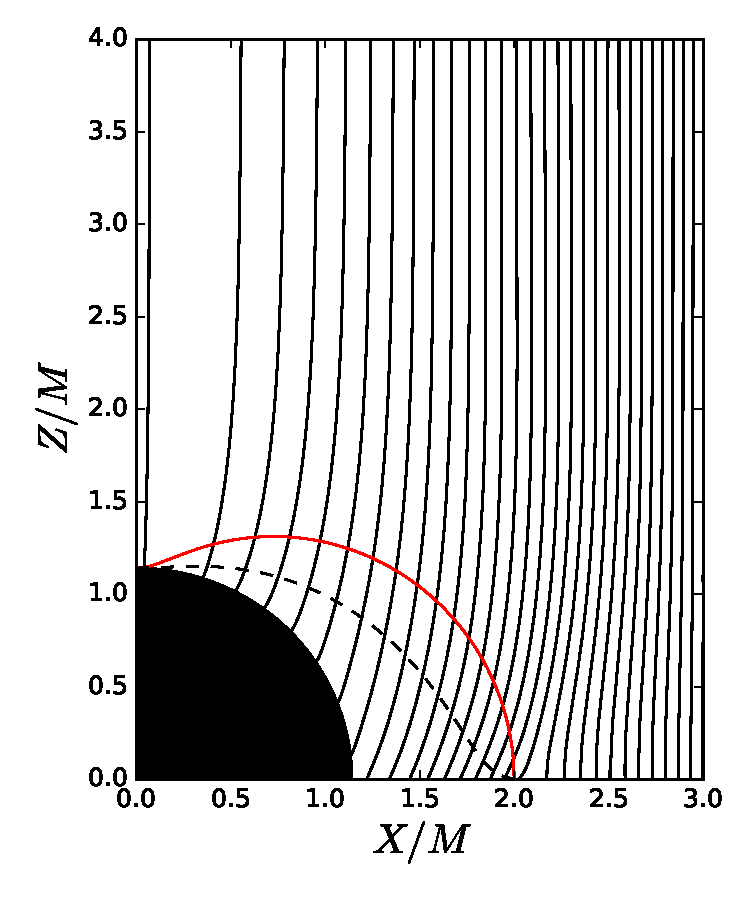
\includegraphics[scale=0.55]{f1}
\caption{\label{fig:field_lines} The configuration of field lines for the magnetosphere of a Kerr BH with spin $a=0.99$,
where the solid/red line is the ergosphere and the dashed/black line is the LS, both of which intersect with
the equator at $r=2 M$. }
\end{figure}

\begin{figure}
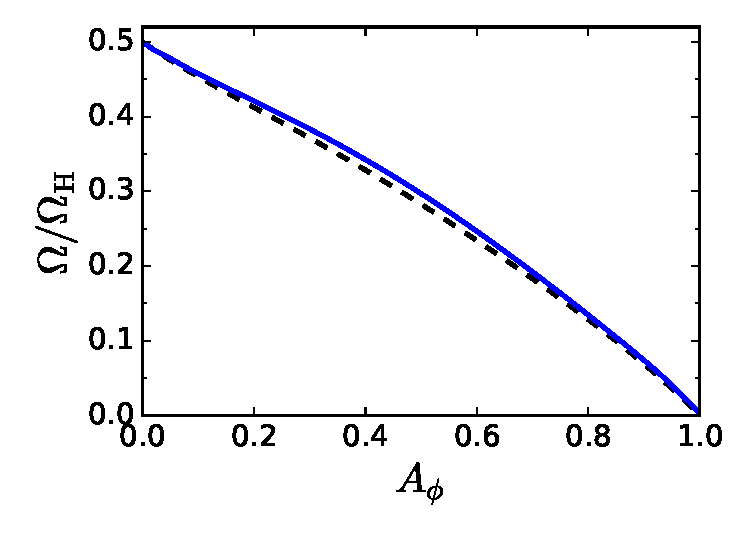
\includegraphics[scale=0.6]{f2}
\caption{\label{fig:omega} $a=0.99$}
\end{figure}

\section{Comparison with previous studies}

\section{Summary and Discussions}

\bibliography{ms}


\end{document}
